\chapter{Binary Instrumentation}
Binary instrumentation is the operation of inserting new code at any point into an existing binary to observe and
possibly modifiy its behaviour; the point at which the new code is added is the \textit{instrumentation point} while the
added instructions are the \textit{instrumentation code}. Binary instrumentation can also be used to improve the
resilience of a binary - e.g. insrumenting {\ttfamily call} and {\ttfamily ret} to ensure that the control flow is
redirected only to a list of expected targets. Instrumenting a binary is no easy task as the insertion of additional
code would normally break all of the references; that's the reason why APIs have been developed to allow the
installation of callbacks at the instrumentation points. Instrumentation tools can be distinguished into static and
dynamic and will be detailed in the following sections.



\section{Static Binary Instrumentation}
Static Binary Instrumentation (SBI hereafter) uses binary rewriting on disks - i.e. the files are actually modified on
disk. SBI tools include PEBIL and Dynisnt (which actually supports bothSBI and DBI). The challenge, as already
mentioned, is to rewrite code without breaking any reference; in order to do so there are two known appproaches:
\begin{itemize}
    \item The {\ttfamily INT3} approach;
    \item The \textit{trampoline} approach.
\end{itemize}


\subsection{The INT3 Approach}
Due to the impossibility to introduce new code without breaking the binary, the additional code must be stored into a
separate location such as a new section or shared library. A possibility would be to substitute the instruction at the
instrumentation point with a {\ttfamily jmp} to the instrumentation code (which must include the originally substituted
instruction in order to maintain consistency in the code). The problem is that if the instrumentation code changes the
content of the registers it will change the program behaviour; thus the SBI tools must save the register state and
restore it at the end of the instrumentation phase (unless registers are voluntarily changed). The problem with this
approach is that normally the {\ttfamily jmp} instruction requires 5 bytes; therefore it is impossible to instrument any
instruction with a length shorter than this without corrupting the following instructions. Furthermore the potentially
corrupted instruction cannot be rewritten into the instrumentation code as it might be the target of a branch
instruction.
\begin{figure}[!htbp]
    \begin{center}
        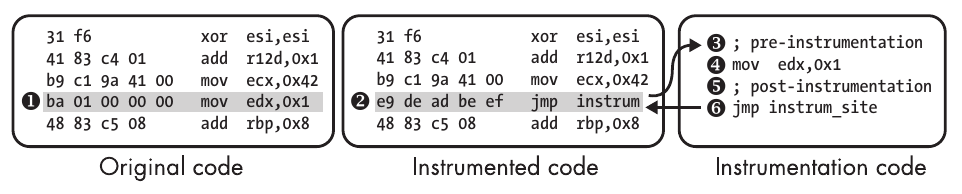
\includegraphics[scale=0.5]{./pics/naive_SBI.png}
        \caption{Naive SBI}
        \label{naive_SBI}
    \end{center}
\end{figure}
The {\ttfamily INT3} instruction, being only 1 byte long resolves the problem of multiple bytes instructions; {\ttfamily
INT3} generates a {\ttfamily SIGTRAP} which is caught by the SBI tool. At this point it becomes possible to use the
{\ttfamily PTRACE} set of functions to gain control of the flow and then execute the instrumented code.


\subsection{The Trampoline Approach}
The trampoline approach uses a completely different technique; the original code is copied and instrumented. In this
case references will not break as the instrumented code will be reached by means of  {\ttfamily jmp}s - i.e. the
\textit{trampolines}; whenever the control is transferred to the original code the trampolines will redirect it to the
corresponding instrumented chunks (which are located into the {\ttfamily .text.instrum}).
\begin{figure}[bpth]
    \begin{center}
        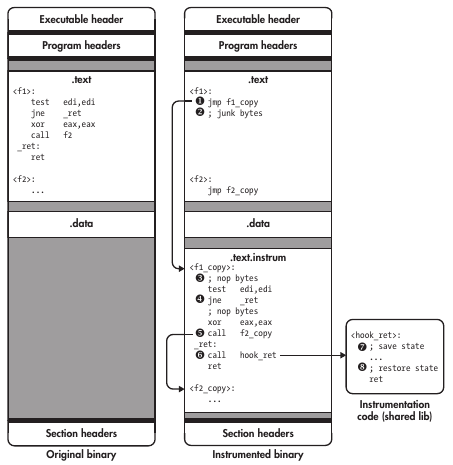
\includegraphics[scale=0.7]{./pics/trampoline.png}
        \caption{Trampoline}
        \label{trampoline}
    \end{center}
\end{figure}
As soon as a function is called the trampoline jumps to its copy; the jump instruction might corrupt the following ones,
but they are never executed in reality. The SBI inserts several {\ttfamily nop}s at the instrumentation points so that
the SBI can overwite them with a jump or a call. The insertion of the instrumentation code and {\ttfamily 0x90} is done
statically. Relative jumps are patched in order to maintain their correctness despite the code shifting caused by the
insertion of code; all of the 2 bytes long jumps, having an 8-bit offset, are replaced with 5 bytes long jumps, with a
32-bit offset, due to the fact that with the additional code 8 bits might not be enough to encode the jumps. The
{\ttfamily call} instructions are rewritten as to redirect the execution on the instrumented copy instead of the
original code. The instrumented code, which can be contained in a shared library, must save the state of the program at
the beginning of the instrumentation and restore it at the end.

\subsubsection{Indirect Control Flow}
Since indirect control flow target instructions at dynamically computed addresses they cannot be computed by the SBI;
this is managed by transferring control to the original code and using trampolines duly inserted in it. 
\paragraph{Indirect Calls} The SBI code does not alter the code that computes the addresses of indirect calls so that
indirect calls maintain the same functions as targets; these contain trampolines which hand the control over to
instrumented code.
\paragraph{Indirect Jumps} The situation is more complicated for indirect jumps; for example {\ttfamily switch}
statements are implemented through \textit{jump tables} containing all of the possible addresses of relevant {\ttfamily
case}s. The indirect jump from one address to the other via the table lands in the original code; due to unexhaustive
basic symbolic information it is really difficult to patch the cases as there is no easy way to understand where the
trampolines are to be placed and there is also the underlying risk of corrupting them should there be not enough space
between one another. Patching the jump table is equally risky as it would be possible to change data that happens to be
a valid address instead.
\paragraph{Position-Indipendent Code} The analysis of PIE code requires special support as they might read the program
counter with instrumented code - i.e. with mutated references - and use it for address computations. In order to
overcome this pitfall SBI instruments the instruction reading the \reg{rip} as to let them return the result that they
would have in the original code.



\section{Dynamic Binary Instrumentation}
